
\documentclass[letterpaper,12pt]{article}
 
\usepackage[spanish]{babel}
\usepackage[utf8]{inputenc}
\usepackage{listings}
\usepackage{graphicx}
 
%%%%%%%%%%%%%%%%%%%%%%%%%%% PORTADA %%%%%%%%%%%%%%%%%%%%%%%%%%%%%%%%%%%%%%%
\makeatletter
\def\thickhrulefill{\leavevmode \leaders \hrule height 1pt\hfill \kern \z@}
\renewcommand{\maketitle}{\begin{titlepage}%
    \let\footnotesize\small
    \let\footnoterule\relax
    \parindent \z@
    \reset@font
    \null\vfil
    \begin{flushleft}    
      \small \@curso \par
      \huge{\textbf{\@title}} \par
    \end{flushleft}
    \par
    \hrule height 4pt
    \par
    \begin{flushright}
      \Huge{\textbf{\@author}} \par
      \bigskip
      \normalsize{\@primerautor} \par
      \normalsize{\@segundoautor} \par
      \bigskip
      \bigskip
      \normalsize \@date \par
    \end{flushright}
    \vskip 60\p@
    \vfil\null
  \end{titlepage}%
  \setcounter{footnote}{0}%
}
\def\primerautor#1{\def\@primerautor{#1}}
\def\segundoautor#1{\def\@segundoautor{#1}}
\def\curso#1{\def\@curso{#1}}
\makeatother
%%%%%%%%%%%%%%%%%%%%%%%%%%% PORTADA %%%%%%%%%%%%%%%%%%%%%%%%%%%%%%%%%%%%%%%
 
 
 
%%%%%%%%%%%%%%%%%%%%%%%%%%% DATOS PERSONALES %%%%%%%%%%%%%%%%%%%%%%%
\curso{CC4102 Dise\~no y An\'alisis de Algoritmos}
\title{Informe Tarea I}
 
\primerautor{Agust\'in L\'opez Q.}
\segundoautor{Mat\'ias Cisterna M.}
 
 
 
\begin{document}
 
\maketitle
 
 
\newpage
\thispagestyle{empty}
\tableofcontents
\setcounter{page}{0}
\newpage
 
\section{Introducci\'on}
En esta tarea 1 de Dise\~no y An\'alisis de Algoritmos se busca analizar sobre una estructura de datos dada (R-tree) diferentes algoritmos de inserci\'on y como estos repercuten en la operaci\'on de b\'usqueda sobre la estructura de datos.
	
Un R-tree es una estructura de datos del tipo \'arbol. Esta estructura es usualmente utilizada para m\'etodos de acceso espacial. Es decir, esta estructura indexa informaci\'on de localizaci\'on, para luego ser consultada de forma eficiente. Consultas del tipo: \textit{encontrar todos los puntos en un radio y centro dado, que cumplan cierto requisito}. La idea de la estructura R-tree es a medida que se inserta y se borra ir manteniendo el \'arbol balanceado y que todos los nodos y hojas cercanos a un dato est\'en localizados espacialmente cerca. Con el fin de lograr que la b\'usqueda de un vecindario de un punto en especial sea eficiente.

\newpage 
\section{Hip\'otesis}
Se cree que \textit{LinearSlpit} va a tomar menos tiempo en las inserciones que \textit{QuadraticSplit}. Sin embargo, al generar un \textit{R-tree} mas irregular su tiempo en la busqueda sera mayor que \textit{QuadraticSplit}. 

\newpage
\section{Dise\~no Experimental}
\subsection{Implementaci\'on}
Para la implementaci\'on se us\'o el lenguaje de programaci\'on Java. El dise\~no se dividi\'o en 6 clases:

\begin{itemize}
\item \textit{RTree}: Representa el \'arbol R-Tree.
\item \textit{Node}: Representa un nodo dentro del \'arbol.
\item \textit{Rectangle}: Representa los rect\'angulos guardados en los nodos.
\item \textit{StopWatch}: Clase creada para medir tiempos de forma simple.
\item \textit{Main}: Clase con m\'etodo \textit{main}, es desde donde se obtiene los datos ficticios.
\item \textit{Data}: Clase que contiene un método \textit{main} el cual se ejecuta para obtener los datos reales.
\end{itemize}

Para la representaci\'on de los rect\'angulos se cre\'o la clase \textit{Rectangle}, donde se guardan como variables de instancia los puntos $(x_1,y_1)$ y $(x_2,y_2)$ los que representan la esquina inferior izquierda y superior derecha, respectivamente. Adem\'as se guarda como variable de instancia una referencia a un nodo, el que puede ser nulo cuando el rect\'angulo es real (rect\'angulo insertado con metodo \textit{insert}), o puede ser un nodo hijo cuando el rect\'angulo es un \textit{MBR}. El objeto \textit{Rectangle} cuenta con m\'etodos para obtener el \'area y saber si dos rect\'angulos se intersectan (para esta parte se considera que si dos rect\'angulos solo comparten un v\'ertice o una arista entonces no se intersectan).
La clase \textit{Node} guarda como variable de instancia una lista con sus rect\'angulos, la variable $t$, una referencia a su nodo padre y una variable booleana que indica si es o no una hoja.
Por su parte la estructura de datos R-Tree guarda los rect\'angulos en sus nodos. La cantidad de rect\'angulos guardados en cada nodo del \'arbol fluctua entre $t$ y $2t$, donde $t$ es definida previamente y depende a su vez de la siguiente condici\'on: \textit{La cantidad de rect\'angulos es tal que, un nodo completo debe caber totalmente dentro de un bloque de memoria}. Para hacer esto se usaron clases provistas por el lenguaje para calcular el tamaño que usar\'ia una estructura \textit{Node} y el hecho de que un bloque tiene tama\~no $4KB$ (4096 bytes).
La implementaci\'on de la estructura de datos consta de dos algoritmos, uno de b\'usqueda y otro de inserci\'on de rect\'angulos.
\begin{itemize}
\item B\'usqueda: El algoritmo de b\'usqueda recibe como par\'ametro un rect\'angulo y retorna una lista con todos los rect\'angulos reales que intersectan a este rect\'angulo. La implementaci\'on es bastante sencilla, pero tiene una pequeña modificaci\'on, no retorna la lista de rect\'angulos que intersectan. Si no que recibe como par\'ametro una lista vac\'ia y esta se va llenando a medida que se encuentre con rect\'angulos que intersectan. Para luego retornar el n\'umero de lecturas/escrituras que hace el algoritmo. Las que son simuladas y contadas cada vez que se accede a un nodo hijo correspondiente a un rect\'angulo MBR que intersecta con el rect\'angulo par\'ametro.
\lstset{language=Java, breaklines=true, basicstyle=\footnotesize}
\begin{lstlisting}[frame=single]
public int searchRectangle(Rectangle r, ArrayList<Rectangle> lst)
  int IOs = 0;
  for(Rectangle nr : rectangles){
    if(!r.equals(nr) && r.intersect(nr)){
      if(isLeaf)
        lst.add(nr);
      else
        IOs += 1 + nr.node.searchRectangle(r,lst);
    }
  }
}
return IOs;
\end{lstlisting}
\item Inserci\'on: Para la inserci\'on se hace un recorrido del \'arbol hasta llegar a una hoja, que es donde se insertar\'a el nuevo rectan\'angulo. El recorrido es como sigue: Se parte de la ra\'iz y se busca el rect\'angulo en su lista que genere el menor incremento de \'area al crear el MBR entre este y el nuevo rect\'angulo. Luego se desciende por el nodo asociado a este rect\'angulo y se hace el mismo procedimiento, hasta llegar a una hoja. Al igual que en la b\'usqueda, en la inserci\'on se hace una modificaci\'on al algoritmo para que este retorne el n\'umero de I/O's que hace a disco. Estas I/O's se cuentan de la siguiente forma: Si el rect\'angulo que est\'a en el nodo no es una hoja, se suma uno a la cantidad total de I/O's y se hace el llamado recursivo. De lo contrario, si es una hoja, se usa un nuevo m\'etodo llamado \textit{insertOverflowedRectangle} el que se encarga de insertar el rect\'angulo y hacer \textit{split} si se produce \textit{overflow}. Para contar la cantidad de I/O's en este m\'etodo se usa la siguiente estrategia: Si despu\'es de insertar no hay \textit{overflow} entonces se retorna 0. De lo contrario primero se verifica si es que estamos en la ra\'iz, de ser as\'i creamos un nuevo nodo. El que ser\'a la nueva ra\'iz y le sumamos uno al total de I/O's. Ya que al crear el nuevo nodo se cuenta una nueva escritura. Luego se verifica cual de los 2 m\'etodos se usara para separar la lista de rect\'angulos y se llama al algoritmo correspondiente (\textit{linearSplit} o \textit{quadraticSlpit}). Luego se aloca en memoria un nuevo nodo (nueva escritura) el que representar\'a al nuevo nodo con la "mitad" de los rect\'angulos del nodo anterior, y se suma uno m\'as a la cantidad de I/O's. Despu\'es se calculan los nuevos MBR de ambos grupos de rect\'angulos y se hace un llamado recursivo por cada rect\'angulo nuevo creado. Para as\'i insertarlos en el nodo padre, y la cantidad de I/O's de estos dos llamados recursivos se suman al total de I/O's que se han acumulado, finalemente llamando al m\'etodo \textit{update} que actualiza todos los MBR desde la hoja hasta el padre.
\end{itemize}
Los dos m\'etodos para separar nodos son heur\'isticas para obtener una separaci\'on lo m\'as \textit{equitativa} posible de los rect\'angulos. A Continuaci\'on se detalla a grandes razgos la implementaci\'on de ambos algoritmos:
\begin{itemize}
\item \textit{QuadraticSplit}: Escogemos los dos rect\'angulos $R_1$ y $R_2$ cuyo incremento de \'area es m\'aximo si es que fueran puestos en el mismo grupo. Es decir, $R_1$ y $R_2$ maximizan (\'area del MBR de $R_1$ y $R_2$) $-$ (\'area de $R_1$ + \'area de $R_2$), sobre todos los pares de rect\'angulos. Asignamos $R_1$ y $R_2$ a grupos distintos.

\lstset{language=Java, breaklines=true, basicstyle=\footnotesize}
\begin{lstlisting}[frame=single]
public void quadraticSplit(ArrayList<Rectangle> g1, ArrayList<Rectangle> g2){
  Rectangle newMBR;
  // indices finales de los rectangulos elegidos para separar en 2 grupos
  int final_i = 0, final_j = 1;
  double incremento = 0.0;
  ArrayList<Rectangle> lst = new ArrayList<Rectangle>();
  // separando en grupos
  for(int i=0;i<rectangles.size()-1;i++){
    lst.add(rectangles.get(i));
    for(int j=i+1; j<rectangles.size();j++){
      lst.add(rectangles.get(j));
      newMBR = makeMBR(lst);
      double newincremento = newMBR.area() - rectangles.get(i).area() - rectangles.get(j).area();
      if(incremento < newincremento){
        incremento = newincremento;
        final_i = i;
        final_j = j;
      }
      lst.remove(rectangles.get(j));
    }
    lst.remove(rectangles.get(i));
  }
  // asignamos a R1 y R2 a grupos distintos
  Rectangle R1 = rectangles.get(final_i);
  Rectangle R2 = rectangles.get(final_j);
  g1.add(R1);
  g2.add(R2);
  rectangles.remove(R1);
  rectangles.remove(R2);

\end{lstlisting}
Iterativamente asignamos un grupo para el resto de los rect\'angulos como sigue:
\begin{itemize}
\item Si todos los rect\'angulos tienen grupo asignado, nos detenemos. Si hay un grupo con tan pocos elementos, que la \'unica forma de que tenga al menos $t$ rect\'angulos es agregando todos los rect\'angulos restantes a este grupo, entonces los agregamos y nos detenemos.
\item Para cada rect\'angulo $R$ que a\'un no tiene grupo, calculamos $g_1$ = incremento en \'area por agregar $R$ al grupo 1. Similarmente, calculamos $g_2$. Escogemos R tal que maximiza $|g_1 - g_2|$. Agregamos $R$ al grupo cuyo incremento en \'area por incluir $R$ es menor. Si hay empate, escogemos el grupo con menor \'area. Si el \'area es la misma, escogemos el grupo con menor cantidad de rect\'angulos. Si sigue habiendo empate, escogemos un grupo arbitrariamente. Volvemos al paso anterior.

\end{itemize}

\item \textit{LinearSlpit}: Se considera un rect\'angulo $R = [x_1, x_2] \times [y_1, y_2]$. El lado menor y mayor de $R$ en la dimensi\'on $x$ es $x_1$ y $x_2$, respectivamente. Similarmente, para la dimens\'on $y$ ser\'a $y_1$ e $y_2$. Escogemos dos rect\'angulos $R_1$ y $R_2$ como sigue: Por cada dimensi\'on $d$, buscamos el rect\'angulo $A_d$ cuyo lado mayor $a_d$ seg\'un $d$ es m\'inimo, y el rect\'angulo $B_d$ cuyo lado menor $b_d$ seg\'un $d$ es m\'aximo. Calculamos $w_d$ como $b_d - a_d$ dividido por el ancho del conjunto en la dimensi\'on $d$. Escogemos $R_1 = A_d$ y $R_2 = B_d$ tal que $w_d$ es m\'aximo, sobre $d = \{x, y\}$. Asignamos $R_1$ y $R_2$ a grupos distintos.

\lstset{language=Java, breaklines=true, basicstyle=\footnotesize}
\begin{lstlisting}[frame=single]
public void linearSplit(ArrayList<Rectangle> g1, ArrayList<Rectangle> g2){
  Rectangle R1, R2;
  /* para ambas dimensiones buscamos el rectangulo Ad cuyo lado mayor ad es minimo
   * y el rectangulo Bd cuyo lado menor bd es maximo
   */
  Rectangle Ax = rectangles.get(0);
  double ax = Ax.x2;
  Rectangle Ay = rectangles.get(0);
  double ay = Ay.y2;
  Rectangle Bx = rectangles.get(0);
  double bx = Bx.x1;
  Rectangle By = rectangles.get(0);
  double by = By.y1;
  for(Rectangle nr : rectangles){
    if(nr.x2 < ax){
      ax = nr.x1;
      Ax = nr;
    }
    if(nr.y2 < ay){
      ay = nr.y1;
      Ay = nr;
    }
    if(nr.x1 > bx){
      bx = nr.x2;
      Bx = nr;
    }
    if(nr.y1 > by){
      by = nr.y2;
      By = nr;
    }
  }
  double anchox = (Bx.x2 < Ax.x2 ? Ax.x2 : Bx.x2) - (Bx.x1 > Ax.x1 ? Ax.x1 : Bx.x1);
  double anchoy = (By.y2 < Ay.y2 ? Ay.y2 : By.y2) - (By.y1 > Ay.y1 ? Ay.y1 : By.y1);
  double wx = (bx - ax)/anchox;
  double wy = (by - ay)/anchoy;
  if(wx > wy){
    if(Ax != Bx){
      R1 = Ax;
      R2 = Bx;
    }else{
      R1 = rectangles.get(0);
      R2 = rectangles.get(1);
    }
  }else{
    if(Ay != By){
      R1 = Ay;
      R2 = By;
    }else{
      R1 = rectangles.get(0);
      R2 = rectangles.get(1);
    }
  }
  g1.add(R1);
  g2.add(R2);
  rectangles.remove(R1);
  rectangles.remove(R2);
\end{lstlisting}

 Para asignar los rect\'angulos restantes hacemos lo siguiente:
\begin{itemize}
\item Si todos los rects\'angulos tienen grupo asignado, nos detenemos. Si hay un grupo con tan pocos elementos, que la \'unica forma de que tenga al menos $t$ rect\'angulos es agreg\'ando todos los rect\'angulos restantes a este grupo, entonces los agregamos y nos detenemos.

\item Escogemos arbitrariamente un rect\'angulo $R$ que no tiene grupo asignado. Agregamos $R$ al grupo cuyo incremento en \'area por incluir $R$ es menor. Si hay empate, escogemos el grupo con menor \'area. Si el \'area es la misma, escogemos el grupo con menor cantidad de rect\'angulos. Si sigue habiendo empate, escogemos un grupo arbitrariamente. Volvemos al paso anterior.
\end{itemize}
\end{itemize}
\subsection{Generaci\'on de Instancias}

El experimento consiste en medir dos tipos de instancias:
\begin{itemize}
\item \textbf{Aleatorias}: Se generan rect\'angulos aleatorios de la siguiente forma: Primero se generan 2 enteros $x_1$ e $y_1$ que se distribuyen uniformemente en el intervalo $[0,500000]$, estos n\'umeros representan la coordenada de la esquina inferior izquierda del rect\'angulo. Luego, $x_2$ se obtiene sumando a $x_1$ un n\'umero aleatorio en el intervalo $[0,100]$ y finalemente se obtiene $y_2$ usando las variables anteriores y asumiendo que el \'area del rect\'angulo debe estar distribuida aleatoriamente en el intervalo $[0,100]$.

\lstset{language=Java, breaklines=true, basicstyle=\footnotesize}
\begin{lstlisting}[frame=single]
static public Rectangle randomRectangle(){
  /* (x1,y1) es la esquina inferior izquierda del rectangulo
   *  la que se obtiene de forma uniformemente aleatoria
   */
  int x1 = randomInt(0,500000);
  int y1 = randomInt(0,500000);
  int x2 = x1 + randomInt(0,100);
  int y2 = y1 + randomInt(0,100)/(x2-x1);
  return new Rectangle(x1,x2,y1,y2);
}
\end{lstlisting}

Con lo anterior se generan dos \'arboles y conjuntos de rect\'angulos de tama\~no $n$, con $n \in \{2^9,2^{12},2^{15},2^{18},2^{21},2^{24}\}$. Cada conjunto se agrega a uno de los \'arboles con uno de los m\'etodos de inserci\'on implementados, el que es elegido a partir de una variable booleana que se pasa como par\'ametro. Al hacer eso se mide el n\'umero de I/O's y el tiempo demorado.

Despu\'es de esto se generan $n/10$ nuevos rect\'angulos y se realizan b\'usquedas, y en estas tambi\'en se obtienen la cantidad de I/O's y el tiempo que se demora en buscar, por cada grupo se obtiene el promedio de estas medidas y su respectiva desviaci\'on est\'andar.


\item \textbf{Datos Reales}: A partir de datos geoespaciales reales obtenidos de US Census Bureau. Se obtuvo el archivo de rutas del Censo del 2011 del estado de California.  A partir de las rutas primarias y secundarias del estado de California se generaron rectángulos mediante el siguiente código:
\lstset{language=Java, breaklines=true, basicstyle=\footnotesize}
\begin{lstlisting}[frame=single]
while( iterator.hasNext() ){
	SimpleFeature feature = iterator.next();
	BoundingBox bounds = feature.getBounds();
	r = new Rectangle(bounds.getMinX(), bounds.getMaxX(), bounds.getMinY(), bounds.getMaxY());
}
\end{lstlisting}

Esto se logro generando \textit{Bounding Boxes} de los datos obtenidos mediante la función \textit{getBounds()} proporcionada por la api de GeoTools. Cabe destacar que la cantidad de rectángulos generados a partir de los datos reales son: 10.482.

Con lo anterior se generaron dos arboles (uno para cada método de inserción). Finalmente se buscan $n/10$ rectángulos aleatoriamente mediante el siguiente código:
\lstset{language=Java, breaklines=true, basicstyle=\footnotesize}
\begin{lstlisting}[frame=single]
while( iterator.hasNext() ){
	SimpleFeature feature = iterator.next();
	BoundingBox bounds = feature.getBounds();
	r = new Rectangle(bounds.getMinX(), bounds.getMaxX(), bounds.getMinY(), bounds.getMaxY());
	count2++;
  	if (count2 == randomNum){
		break;
  	}
}
\end{lstlisting}

Siendo $n$ la cantidad de rectángulos totales obtenidos de los datos reales. Con ello se obtienen todos los datos necesarios para hacer el análisis posterior.

\end{itemize}



\subsection{Medidas de Rendimiento}
Las medidas de rendimiento usadas son dos:
\begin{itemize}
\item La cantidad de I/O's hechas por una inserci\'on o b\'usqueda. Estas son simuladas en ambos algoritmos. Es decir, en la b\'usqueda cada vez que se accede a un nuevo nodo hijo se suma uno a la cantidad total de I/O's, y no se agregan por escrituras ya que solo se lee. Por otro lado, para las inserciones se suma uno a la cantidad total de I/O's cada vez que se baja en un nivel en el \'arbol. Esto se debe a que hay una nueva lectura de un nodo, adem\'as se suma uno cada vez que hay \textit{overflow}, ya que se genera una nueva escritura (generar nuevo nodo hermano). Por lo tanto tambi\'en se suma uno m\'as extra si hay \textit{overflow} en la ra\'iz, ya que debe haber una nueva escritura al crear un nuevo nodo para la ra\'iz.
	
\item El tiempo de ejecuci\'on de cada operaci\'on. Para esto se cre\'o la clase \textit{StopWatch}, la que se puede iniciar y pausar. Esta incrementa el tiempo total de la ejecución sin ser molestado por ejecuciones de otras partes del c\'odigo.
\end{itemize}
Finalmente estas medidas, tanto de b\'usqueda como de inserci\'on, son almacenadas en un nuevo archivo. Creado con el objetivo de almacenar los datos y luego analizarlos.

\newpage
\section{Presentaci\'on de Resultados}

\subsection{Datos Reales}

\subsubsection{Inserciones}
A continuaci\'on se presenta en una tabla los resultados del experimento de inserci\'on de rect\'angulos generados de datos reales en un R-Tree con el m\'etodo de \textit{QuadraticSplit}: \\
\begin{tabular}{|c|c|c|}
\hline
\textbf{Tama\~no} & \textbf{Cantidad I/O's} & \textbf{Tiempo (milisegundos)} \\
\hline
10482 & 30296 & 191 \\
\hline
\end{tabular}
\\ \\

A continuaci\'on se presenta en una tabla los resultados del experimento de inserci\'on de rect\'angulos generados de datos reales en un R-Tree con el m\'etodo de \textit{LinearSplit}: \\
\begin{tabular}{|c|c|c|}
\hline
\textbf{Tama\~no} & \textbf{Cantidad I/O's} & \textbf{Tiempo (milisegundos)} \\
\hline
10482 & 30058 & 58 \\
\hline
\end{tabular}
\\ \\

\subsubsection{Búsqueda}
A continuaci\'on se presenta en una tabla los resultados del experimento de búsqueda de rect\'angulos generados de datos reales en un R-Tree en el arbol generado con el m\'etodo de \textit{QuadraticSplit}: \\
\begin{tabular}{|c|c|c|}
\hline
\textbf{Tama\~no} & \textbf{Cantidad promedio de I/O's} & \textbf{Tiempo promedio (milisegundos)} \\
\hline
10482 & 0.011450381679389313 & 0.004770992366412214 \\
\hline
\end{tabular}
\\ \\

A continuaci\'on se presenta en una tabla los resultados del experimento de búsqueda de rect\'angulos generados de datos reales en un R-Tree en el arbol generado con el m\'etodo de \textit{LinearSplit}: \\
\begin{tabular}{|c|c|c|}
\hline
\textbf{Tama\~no} & \textbf{Cantidad promedio de I/O's} & \textbf{Tiempo promedio (milisegundos)} \\
\hline
10482 & 0.0 & 0.004770992366412214 \\
\hline
\end{tabular}
\\ \\

\subsection{Datos Generados}
\subsubsection{Inserciones}
A continuación se presenta en una tabla los resultados del experimento de inserción de rectángulos aleatorios en un R-Tree con el método de \textit{QuadraticSplit}: \\
\begin{tabular}{|c|c|c|}
\hline
\textbf{Tama\~no ($2^n$)} & \textbf{Cantidad I/O's} & \textbf{Tiempo (milisegundos)} \\
\hline
9 & 755 & 43 \\
\hline
12 & 10656 & 115 \\
\hline
15 & 118832 & 1043 \\
\hline
18 & 1193602 & 9624 \\
\hline
21 & 11553820 & 84628 \\
\hline
24 & 141142799 & 476308 \\
\hline
\end{tabular}
\\ \\
Los gr\'aficos de ambos datos, en escala logar\'itmica para su mejor visualizaci\'on se encuentran en la Figura~\ref{fig:f1} y ~\ref{fig:f2}.

Ahora se presenta en una tabla los resultados del experimento de inserción de rectángulos aleatorios en un R-Tree con el método de \textit{LinearSplit}: \\
\begin{tabular}{|c|c|c|}
\hline
\textbf{Tama\~no ($2^n$)} & \textbf{Cantidad I/O's} & \textbf{Tiempo (milisegundos)} \\
\hline
9 & 740 & 23 \\
\hline
12 & 10471 & 36 \\
\hline
15 & 113245 & 451 \\
\hline
18 & 1192441 & 4683 \\
\hline
21 & 11118402 & 46764 \\
\hline
24 & 136824746 & 252177 \\
\hline
\end{tabular}

Los gr\'aficos de ambos datos, en escala logar\'itmica para su mejor visualizaci\'on se encuentran en la Figura~\ref{fig:f3} y ~\ref{fig:f4}.

\subsubsection{Búsqueda}
A continuación se presenta en una tabla los resultados del experimento de busqueda de rectángulos aleatorios en un R-Tree con el método de inserción \textit{QuadraticSplit}: \\
\begin{tabular}{|c|c|c|}
\hline
\textbf{Tama\~no ($2^n$)} & \textbf{Cantidad promedio de I/O's} & \textbf{Tiempo promedio (milisegundos)} \\
\hline
9 & 0.0 & 0.0 \\
\hline
12 & 0.0 & 0.0 \\
\hline
15 & 0.0 & 0.0 \\
\hline
18 & 0.0 & 7.629510948348211E-5 \\
\hline
21 & 0.0 & 3.337863290656367E-5 \\
\hline
24 & 0.0 & 2.384186643667213E-5 \\
\hline
\end{tabular}
\\ \\

A continuación se presenta en una tabla los resultados del experimento de busqueda de rectángulos aleatorios en un R-Tree con el método de inserción \textit{LinearSplit}: \\
\begin{tabular}{|c|c|c|}
\hline
\textbf{Tama\~no ($2^n$)} & \textbf{Cantidad promedio de I/O's} & \textbf{Tiempo promedio (milisegundos)} \\
\hline
9 & 0.0 & 0.0 \\
\hline
12 & 0.0 & 0.0024449877750611247 \\
\hline
15 & 0.0 & 9.157509157509158E-4 \\
\hline
18 & 0.0 & 1.1444266422522316E-4 \\
\hline
21 & 0.0 & 4.291538516558186E-5 \\
\hline
24 & 0.0 & 2.7418146402172948E-5 \\
\hline
\end{tabular}
\\ \\




\newpage
\subsection{Gráficos}

\begin{figure}[bp!]
  \centering
    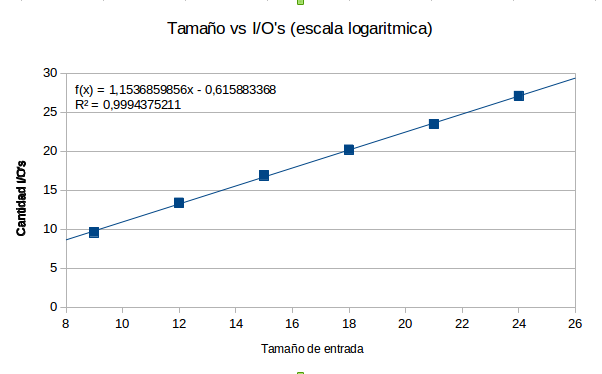
\includegraphics[width=0.8\textwidth]{quadratic_io}
  \caption{Gr\'afico Tama\~no vs I/O's para QuadraticSplit}
  \label{fig:f1}
\end{figure}

\begin{figure}[bp!]
  \centering
    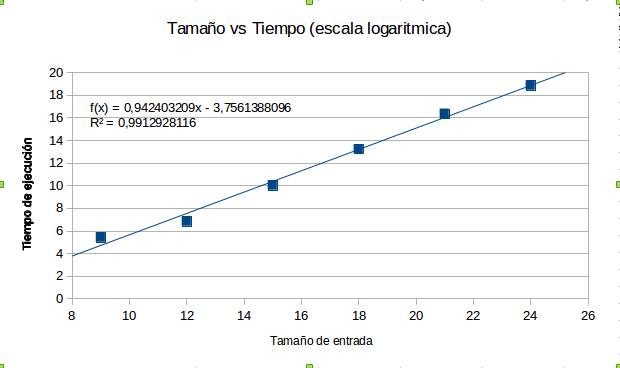
\includegraphics[width=0.8\textwidth]{quadratic_tiempo}
  \caption{Gr\'afico Tama\~no vs Tiempo para QuadraticSplit}
  \label{fig:f2}
\end{figure}

\begin{figure}[bp!]
  \centering
    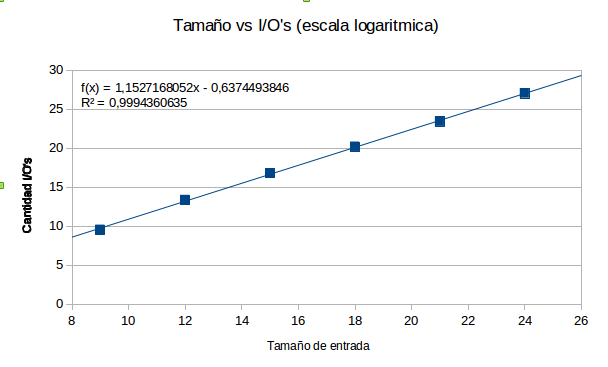
\includegraphics[width=0.8\textwidth]{linear_io}
  \caption{Gr\'afico Tama\~no vs I/O's para LinearSplit}
  \label{fig:f3}
\end{figure}

\begin{figure}[bp!]
  \centering
    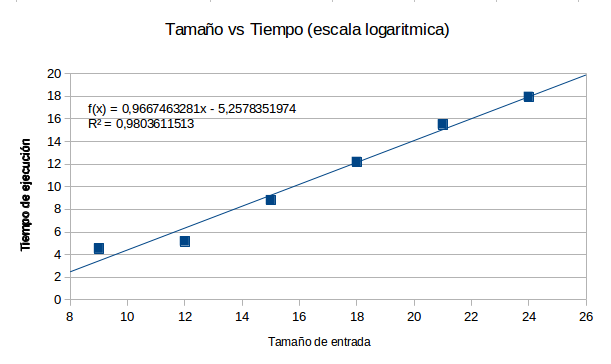
\includegraphics[width=0.8\textwidth]{linear_tiempo}
  \caption{Gr\'afico Tama\~no vs Tiempo para LinearSplit}
  \label{fig:f4}
\end{figure}

\newpage
\section{An\'alisis e Interpretaci\'on de Datos}
 \subsection{Inserciones}
 
Podemos ver que para el caso de datos generados la cantidad de I/O's y el tiempo a medida que crece $n$, es lineal para ambos casos de inserción(\textit{LinearSplit} y \textit{QuadraticSplit}). Sin embargo, podemos notar que para el caso de \textit{LinearSplit} este toma casi la mitdad del tiempo que \textit{QuadraticSplit}. Ademas \textit{LinearSplit} hace ligeramente menos I/O's que \textit{QuadraticSplit}.

Por otro lado, en el caso en que los rectángulos son generados a partir de datos reales. Vemos que nuevamente el tiempo de inserción para el método \textit{LinearSplit} toma bastante menos tiempo que textit{QuadraticSplit}. Sin embargo, en la cantidad de I/O's ambos algoritmos se comportan relativamente similar.

Dado la naturaleza de ambos algoritmos de inserción es fácil ver que para el caso de \textit{LinearSplit} este iba a lograr menores tiempos de inserción en comparación a \textit{QuadraticSplit}. Esto se debe a que la naturaleza de su algoritmo hace generar arboles mas irregulares. Es decir, genera arboles menos balanceados que \textit{QuadraticSplit}. Esto se debe a que las estrategias de \textit{LinearSplit} son mas laxas. Sin embargo, esto puede producir que al momento de realizar operaciones sobre un árbol generado por \textit{LinearSplit} esta tome mas tiempo que en \textit{QuadraticSplit}.

 
\subsection{Búsqueda}
Lamentablemente después de analizar ambos casos, Datos reales y generados. Se puede concluir que el método de búsqueda posee algún error. Se cree que este no estaba cargando los datos de disco por lo tanto al leerlos de memoria primaria arroja los datos adjuntos. Que son de costo prácticamente cero para ambos casos, que es de esperarse si los datos son leídos de memoria primaria.  

Por otro lado se esperaba que \textit{QuadraticSplit} tuviese mejores tiempos y menores I/O's que \textit{LinearSplit}.
 
\end{document}
